\documentclass{layout/TU-Delft-report}

% ----------------------------- %
% Custom Commands
% ----------------------------- %

\RenewCommandCopy\qty\SI  % Redefine \qty to use \SI

% Reference Formatting
\newcommand{\tableme}[1]{Table: \ref{#1}}
\newcommand{\figref}[1]{Figure: \ref{#1}}


% ----------------------------- %
% Package Imports
% ----------------------------- %

% Essential Formatting Packages

\let\openbox\relax
\usepackage{amsthm}
\usepackage[bottom]{footmisc}
\usepackage{dirtytalk}
\usepackage{printlen}
\usepackage[percent]{overpic}

\usepackage[lines=4]{lettrine}
\usepackage{cases}
\usepackage{hyperref}
\usepackage{wrapfig}
\newtheorem{theorem}{Theorem}
\newtheorem{corollary}[theorem]{Corollary}
\newtheorem{lemma}[theorem]{Lemma}
\usepackage{subcaption}
\newtheorem{definition}{Definition}
\usepackage{xcolor}
\definecolor{delft_blue_shade1}{RGB}{12,35,64}
\definecolor{royal_blue}{RGB}{0, 118, 194}
\definecolor{delft_blue_shade2}{RGB}{229,246,251}
\usepackage{parskip}  % Adjust paragraph spacing
\usepackage{multicol} % Multiple columns
\usepackage{adjustbox} % Adjusting table and figure sizes
\usepackage{booktabs} % Better table formatting
\usepackage{rotating} % Rotating figures and tables
\usepackage{hhline} % Advanced table lines
\usepackage{multirow} % Multi-row tables
\usepackage{tabularx} % Advanced table layout
\usepackage[graphicx]{realboxes} % Rotating text in tables
\usepackage{colortbl} % Colored tables
\usepackage{psfrag} % Replace text in figures
\usepackage{balance} % Balancing columns in two-column mode
\usepackage{url}
\usepackage{threeparttable}
\usepackage{booktabs} 
\usepackage{bbm}
\usepackage{eurosym}

% Algorithm & Pseudocode Packages
\usepackage[linesnumbered,ruled,vlined]{algorithm2e}
\SetKwInput{KwInput}{Input} % Set input format
\SetKwInput{KwOutput}{Output} % Set output format
\usepackage{algpseudocode}
\let\listofalgorithms\relax
\usepackage{algorithm}

% Math & Symbols
\usepackage{amssymb}
\usepackage[nocomma]{optidef} % Optimization notation
\usepackage{nomencl} % Nomenclature package
\makenomenclature
\usepackage{etoolbox} % Required for nomenclature grouping
\renewcommand\nomgroup[1]{%
  \item[\itshape
  \ifstrequal{#1}{A}{Sets}{%
  \ifstrequal{#1}{B}{Indices}{%
  \ifstrequal{#1}{C}{Parameters}{
  \ifstrequal{#1}{D}{Variables}
  }}}]}
\newcommand{\tugradientdot}{
  \begin{center}
    \begin{tikzpicture}[baseline]
      % Left gradient line
      \shade[left color=gray!50, right color=gray!10]
        (-6,0) rectangle (0,0.2);
      % Center dot
      \node at (0.5,0) {\textbullet};
      % Right gradient line
      \shade[left color=gray!10, right color=gray!50]
        (1,0) rectangle (7,0.2);
    \end{tikzpicture}
  \end{center}
}

% Citations & References
\usepackage[numbers]{natbib}
\usepackage[printonlyused]{acronym}
%% Chapter - 3
\usepackage{nomencl}
\makenomenclature
%% This code creates the groups
% -----------------------------------------
\usepackage{etoolbox}

\newcommand{\Drawlegend}[6]{% linewidth, length, color,dashed/solid, marker(0 or 1), markersize
  \begin{tikzpicture}[baseline=-3pt]
    \draw[line width=#1, color=#3, #4] (0,0) -- (#2,0);
    \fill[color=#3] (#2/2,0) circle [radius=#5*#6/2];
  \end{tikzpicture}%
}


\let\WriteBookmarks\relax
\def\floatpagepagefraction{1}
\def\textpagefraction{.001}

% Color Definitions
\definecolor{c1}{HTML}{fc8d59}
\definecolor{c2}{HTML}{ef6548}
\definecolor{c3}{HTML}{d7301f}
\definecolor{c4}{HTML}{b30000}
\definecolor{c5}{HTML}{7f0000}

\usepackage{tikz,lipsum,lmodern}
\usepackage[most]{tcolorbox}
\usepackage{amsmath,amssymb}

\usepackage{array} % required for text wrapping in tables

\newcommand{\redDashedLine}{\textcolor{red}{\rule[0.5ex]{.2em}{0.8pt}\hspace{0.2em}\rule[0.5ex]{.2em}{0.8pt}\hspace{0.2em}\rule[0.5ex]{.2em}{0.8pt}\hspace{0.2em}\rule[0.5ex]{.2em}{0.8pt}}}

\makeatletter
\newcommand{\printtitle}{\@title}
\makeatother

\newcommand{\blackDashedLine}{\textcolor{black}{\rule[0.5ex]{.2em}{0.8pt}\hspace{0.2em}\rule[0.5ex]{.2em}{0.8pt}\hspace{0.2em}\rule[0.5ex]{.2em}{0.8pt}\hspace{0.2em}\rule[0.5ex]{.2em}{0.8pt}}}
%% Chapter design parameters
% \usepackage[Lenny]{fncychap}

%%----------------------------------------
%% Keywords new command
%%----------------------------------------
\newtcbox{\keywordtag}{
  on line,
  colback=delft_blue_shade2,
  colframe=royal_blue,
    boxrule=.1pt,
  arc=1mm,
  boxsep=1pt,
  left=8pt, right=8pt,
  top=2pt, bottom=2pt,
  height=2.5em,           % �� fixes total box height
  valign=center,          % centers text inside
  fontupper=\sffamily\color{royal_blue},
  enhanced
}

\def\headline#1{\hbox to \hsize{\hrulefill\quad\lower.5pt\hbox{#1}\quad\hrulefill}}


% ----------------------------- %
% Hyperref Setup
% ----------------------------- %
\hypersetup{
    colorlinks=true,
    linkcolor=blue,
    filecolor=magenta,      
    urlcolor=cyan,
    pdftitle={Overleaf Example},
    pdfpagemode=FullScreen,
}


\urlstyle{same}
%%%%%%%%%%%%%%%%%%%%%%%%%%%%%
%%%%% Begin of document %%%%%
%%%%%%%%%%%%%%%%%%%%%%%%%%%%%

\begin{document}



%% Roman page numbering
\frontmatter

%% Defining the main parameters

\title{\textbf{My PhD Thesis}}

\subtitle{PhD Thesis Template (2025) for \LaTeX} 

\author{N. K. (Nanda) Panda}
\subject{Delft University of Technology }
\affiliation{Delft University of Technology}
\coverimage{figures/cover_page.pdf} % Aspect ratio of 2:3 (portrait) recommended
\definecolor{title}{HTML}{4884d6} % Color for title
\makecover
\begin{titlepage}

\begin{center}
\printtitle \\ ~\\~\\~\\~\\~\\%< Title of dissertation>
Dissertation \\ ~\\~\\
for the purpose of obtaining the degree of doctor \\
Delft University of Technology  \\
by the authority of the Rector Magnificus, prof.dr.ir. X.Y.Z. van at London,\\%<titles, name>
chair of the Board for Doctorates\\
to be defended publicly on\\
Monday 4 June 2018 at 12:30 o’clock \\~\\ %<date= weekday (word) day (number), month (word) year (number)> at <hh:mm (number)> o’clock
by\\~\\
John Doe\\ %<first names in full and SURNAME in upper case>
Diplom-Informatiker, Technische Universität Darmstadt, Germany%<highest academic title, name university, country>
born in Nowhereland, Habitat %[town/city, country of birth]
\end{center}
\vfill
\end{titlepage}

%*Example diploma not in Latin script:Peng WANGMaster of Engineering in Mathematics, Wuhan University, China
% born in Beijing, China

% *Example Dutch diploma:Ahmad AWAZMaster of Science in Aerospace Engineering, Delft University of Technology, the Netherlands
% born in Jakarta, Indonesia
\begin{titlepage}

This dissertation has been approved by the promotors.

\vspace{1em}
Composition of the doctoral committee:

\begin{tabular}{@{}ll}
Rector Magnificus, & chairperson \\
Prof.dr.ir. P.H.T. Verstappen & Delft University of Technology, promotor \\
Dr.ir. P.D. Deneuve & Delft University of Technology, copromotor \\
\end{tabular}

\vspace{1em}
Independent members:

\begin{tabular}{@{}ll}
Prof.dr.ir. G.M. Van Bekhoven & Delft University of Technology \\
Prof. Y. Ishihara & Tokyo University, Japan \\
Prof.dr. P.M. Charlier & Eindhoven University of Technology \\
Prof.dr.ir. P.L.W. Goncalves Fernandes & Middle East Technical University, Turkey \\
Prof.dr. P. Dijkstra & Delft University of Technology, reserve member \\
\end{tabular}
%% Only include the following 3 lines if confidentiality is applicable.
\bigskip
\bigskip

\emph{This thesis is confidential and cannot be made public until December 31, 2024.}
%\emph{Op dit verslag is geheimhouding van toepassing tot en met 31 december 2024.}

% Place to put ur project, or funding agency logos
\begin{figure}[h]
  \begin{minipage}{0.2\textwidth}
    \fbox{\rule{0pt}{1.5cm}\rule{1.5cm}{0pt}} % placeholder replace by  \includegraphics[width=2cm,height=2cm]{image1.png} % replace placeholder
  \end{minipage}
  \begin{minipage}{0.2\textwidth}
    \fbox{\rule{0pt}{1.5cm}\rule{1.5cm}{0pt}} % placeholder replace by  \includegraphics[width=2cm,height=2cm]{image1.png} % replace placeholder
  \end{minipage}
\end{figure}

Keywords: keyword1, keyword2, keyword3, keyword4\\
Printed by: <company that you printed>\\
Cover: N.K.P 2025 under C.C.  \\ % Example
% Feel free to remove the following attribution, it is not required - still appreciated :-)
Style: TU Delft PhD Thesis Template (2025) for \LaTeX by N.K. Panda \\
Copyright \textcopyright 2025 N.K. Panda \\ % Change this based on the name
ISBN XXX.XX.XXXX.XXXX

\bigskip
\bigskip

An electronic version of this thesis is available at \url{http://repository.tudelft.nl/}.

%% Insert the TU Delft logo at the bottom of the page
\begin{tikzpicture}[remember picture, overlay]
    \node[above=10mm] at (current page.south) {%
        
\includegraphics{layout/tudelft/logo-black}
    };
\end{tikzpicture}
\end{titlepage}







\tableofcontents

\chapter{Abbreviations} %
\begin{acronym}[ACM]
    \acro{EV}{Electric Vehicle}
\end{acronym}


%% Arabic page numbering
\mainmatter
\chapter{Introduction}
\label{chapter-1}
\vfill
\begin{center}
    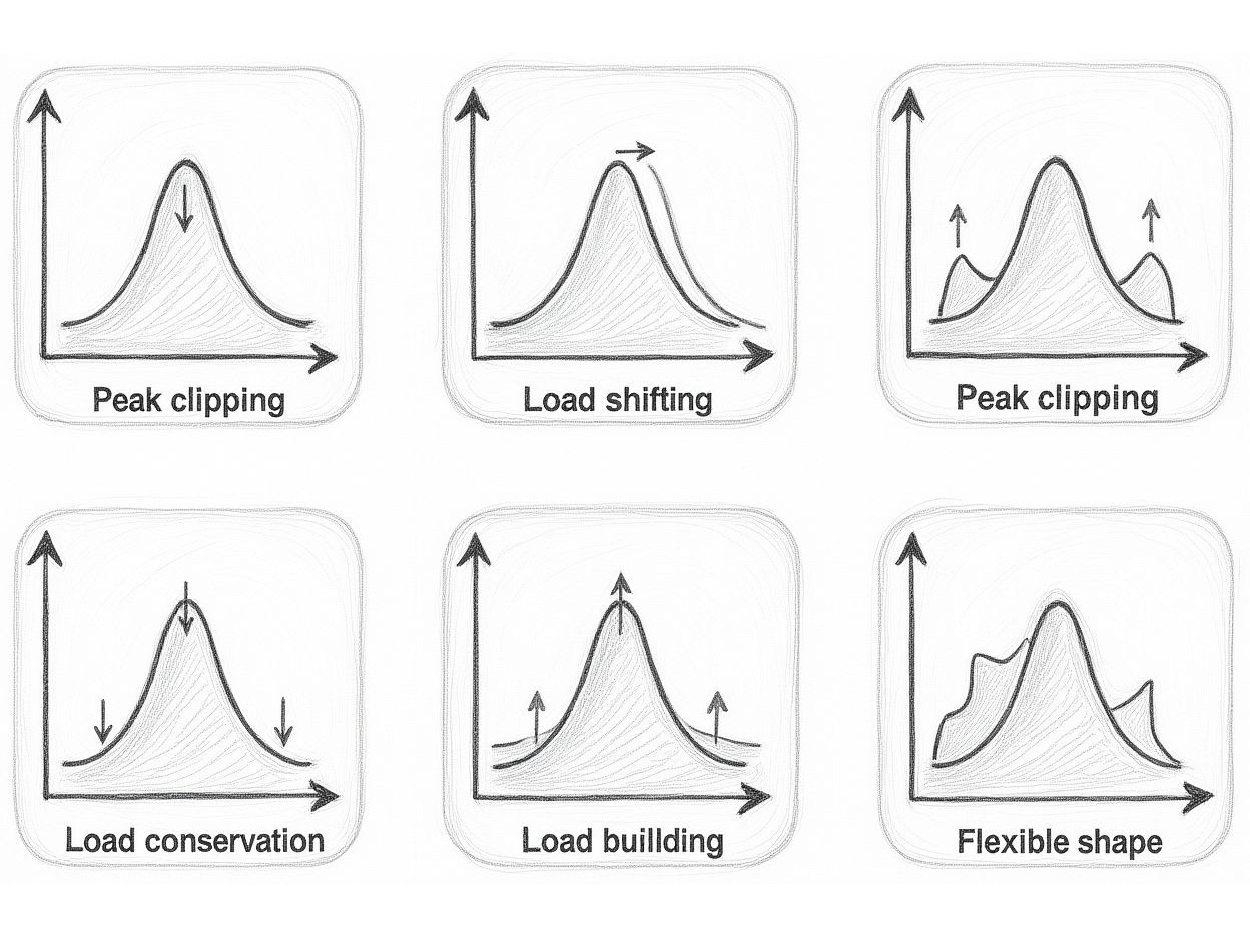
\includegraphics[width=\textwidth]{figures/chapter_1/type_flex_sketch.pdf}
\end{center}
\newpage
% These can be used to do keywords
\section{Different design for putting keywords}
\subsection{One row}
\noindent
K\ E\ Y\ W\ O\ R \ D\ S

\noindent
\keywordtag{Congestion} \hfill
\keywordtag{Flexibility} \hfill
\keywordtag{Smart Charging} \hfill
\keywordtag{Market Product}

\vspace{1 em}
\noindent
\subsection{Multiple row with vertical heading}

\begin{minipage}[b]{0.075\linewidth} 
  \rotatebox[origin=l]{90}{K\ E\ Y\ W\ O\ R \ D\ S \rule{2cm}{0.4pt}} 
\end{minipage}%
\begin{minipage}[b]{0.9\linewidth} % 65% width
\keywordtag{Aggregate Charging}\\
\vspace{0.5 pt}\\
\keywordtag{Congestion} \\
\vspace{0.5 pt}\\
\keywordtag{Electric Vehicles}\\
\vspace{0.5 pt}\\
\keywordtag{Flexibility} \\
\vspace{0.5 pt}\\
\keywordtag{Smart Charging} \\
\end{minipage}
\subsection{Multiple row with horizontal heading}
K\ E\ Y\ W\ O\ R \ D\ S \hrulefill

\noindent
\keywordtag{Aggregate Charging}\\
\vspace{0.5 pt}\\
\keywordtag{Congestion} \\
\vspace{0.5 pt}\\
\keywordtag{Electric Vehicles}\\
\vspace{0.5 pt}\\
\keywordtag{Flexibility} \\
\vspace{0.5 pt}\\
\newpage
\section{Chapter summary style}
\subsection{Horizontal heading}

O\ V\ E\ R\ V\ I\ E\ W \hrulefill\\
\lettrine{\color{royal_blue}E}{nergy} i\lipsum[5]
\subsection{Vertical heading}
\begin{minipage}[b]{0.075\linewidth} 
  \rotatebox[origin=l]{90}{O\ V\ E\ R\ V\ I\ E\ W \rule{2cm}{0.4pt}} 
\end{minipage}%
\begin{minipage}[b]{0.9\linewidth} % 65% width
\lettrine{\color{royal_blue}E}{nergy} \lipsum[8]
\end{minipage}

 

 \vfill
\rule{\textwidth}{0.4pt}
Here you can use this space to refer to the publication on which the following chapter is based. For example, the contents of this chapter are related to the publication: Panda, N. K., \& Tindemans, S. H. (2024). \textit{Quantifying the Aggregate Flexibility of Electric Vehicles Charging Stations for Dependable Congestion Management Products - A Dutch Case Study. \textit{arXiv preprint} \href{https://arxiv.org/abs/2403.13367}{arXiv:2403.13367}.}
\newpage
\section{Using abbreviations}
To streamline the use of abbreviations, it is recommended to use the \say{acronym} package. Then you can write abbreviations like \ac{EV} by defining at a single point as inside the acronym\_list.tex under frontmatter. Plural form of the abbreviation can be written as \acp{EV}, and the full form can be called as \acf{EV}.
\section{Using text box}
To highlight a certain concept, you can use a text box, such as:
\begin{tcolorbox}[colback=delft_blue_shade2,colframe=delft_blue_shade1,title=\textbf{Congestion}]
\begin{wrapfigure}{r}{0.3\linewidth}
    \centering
    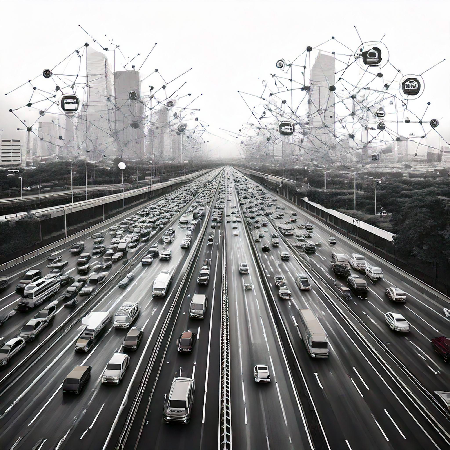
\includegraphics[width=1\linewidth]{figures/chapter_1/congestion_clip_art.pdf}
\end{wrapfigure}
\lipsum[8]
\end{tcolorbox}
\section{Using reference}
Things can be cited like \cite{panda2024aggregate}. Then it will automatically be shown in the Bibliography, provided a supporting \say{.bib} file is supplied. Make sure not to have duplicate entries in the file. 
\section{Section 4}
\lipsum[5]


% Add bibliography
\bibliographystyle{IEEEtran}

\bibliography{references.bib}
\appendix

\chapter{Source Code Example}
%\label{chapter:title}

\emph{Adding source code to your report/thesis is supported with the package {\normalfont\texttt{listings}}. An example can be found below. Files can be added using \\
\texttt{\textbackslash lstinputlisting[language=<language>]\{<filename>\}}}

\begin{lstlisting}[language=Python]
"""
ISA Calculator: import the function, specify the height and it will return a
list in the following format: [Temperature,Density,Pressure,Speed of Sound].
Note that there is no check to see if the maximum altitude is reached.
"""

import math
g0 = 9.80665
R = 287.0
layer1 = [0, 288.15, 101325.0]
alt = [0,11000,20000,32000,47000,51000,71000,86000]
a = [-.0065,0,.0010,.0028,0,-.0028,-.0020]

def atmosphere(h):
    for i in range(0,len(alt)-1):
        if h >= alt[i]:
            layer0 = layer1[:]
            layer1[0] = min(h,alt[i+1])
            if a[i] != 0:
                layer1[1] = layer0[1] + a[i]*(layer1[0]-layer0[0])
                layer1[2] = layer0[2] * (layer1[1]/layer0[1])**(-g0/(a[i]*R))
            else:
                layer1[2] = layer0[2]*math.exp((-g0/(R*layer1[1]))*(layer1[0]-layer0[0]))
    return [layer1[1],layer1[2]/(R*layer1[1]),layer1[2],math.sqrt(1.4*R*layer1[1])]
\end{lstlisting}

\chapter{TU Delft Title Page Guide}
\textbf{The following guideline is based on the official regulations of the Graduate School of TU Delft. It was last updated on 23 September 2025. No rights can be derived from this document. Candidates are strongly advised to consult the most recent guidelines and adapt accordingly. The current version can be found at} % https://filelist.tudelft.nl/me/Onderzoek/Graduate%20School/Documents%20%26%20Links/TUD%20GS%20Title%20page%20guide.pdf
\section*{Making the title page for your doctoral dissertation – a practical guide}

\subsection*{Contents}
1. Introduction, rules and procedure \\
2. The front of the title page \\
3. The reverse side – the basics \\
\quad 3.1 Adding the (co)promotor(s) and chairman \\
\quad 3.2 Adding the committee members \\
\quad 3.3 Other additions \\
4. The end result \\
5. Dual Degree dissertation – reverse side

\section*{1. Introduction, rules and procedure}
Each TU Delft doctoral dissertation must contain a title page containing a standard formula and a number of variables.  
You can find the formal regulations concerning the title page in section D of the Implementation Decree on Doctoral Regulations on the Graduate School website.  

Approval of the title page: when you submit the draft dissertation, propositions and Form B, the title page should also be included. Some variables (such as the defence date and the composition of your doctoral committee) may be left blank initially. Later, after confirmation and approval, the completed title page may be printed.

\section*{2. Front of the title page}
\begin{itemize}
\item May be in English or Dutch (preferably the same as the dissertation).  
\item Text is centered.  
\item Rector Magnificus per 1-1-2018: Prof.dr.ir. T.H.J.J. van der Hagen. Always check the current Rector’s name.  
\item Last name(s) in capitals.  
\item Academic title + university + country must be mentioned.  
\end{itemize}

\subsection*{Template in English}
\begin{center}
[Title of dissertation] \\[1em]
Dissertation \\[1em]
for the purpose of obtaining the degree of doctor \\[0.5em]
at Delft University of Technology \\[0.5em]
by the authority of the Rector Magnificus, [titles, name], \\[0.5em]
chair of the Board for Doctorates \\[1em]
to be defended publicly on \\[0.5em]
[weekday day month year] at [hh:mm] o’clock \\[1em]
by \\[1em]
[FIRST NAMES SURNAME in capitals] \\[0.5em]
[highest academic title, university, country] \\[0.5em]
born in [town/city, country of birth]
\end{center}

\subsection*{Template in Dutch}
\begin{center}
[Titel van het proefschrift] \\[1em]
Proefschrift \\[1em]
ter verkrijging van de graad van doctor aan de Technische Universiteit Delft, \\[0.5em]
op gezag van de Rector Magnificus, prof. [titels, naam], \\[0.5em]
voorzitter van het College voor Promoties, \\[1em]
in het openbaar te verdedigen op \\[0.5em]
[weekdag dag maand jaar] om [uu:mm] uur \\[1em]
door \\[1em]
[VOORNAMEN ACHTERNAAM in hoofdletters] \\[0.5em]
[academische titel, universiteit, land] \\[0.5em]
geboren te [plaats, land]
\end{center}

\subsection*{Examples in English}
\begin{center}
Sustainable concrete infrastructure design \\[1em]
Dissertation \\[1em]
for the purpose of obtaining the degree of doctor \\[0.5em]
at Delft University of Technology \\[0.5em]
by the authority of the Rector Magnificus prof.dr.ir. T.H.J.J. van der Hagen \\[0.5em]
chair of the Board for Doctorates \\[1em]
to be defended publicly on \\[0.5em]
Monday 4 June 2018 at 12:30 o’clock \\[1em]
by \\[1em]
Özlem GÜL \\[0.5em]
Diplom-Informatiker, Technische Universität Darmstadt, Germany \\[0.5em]
born in Munich, Germany
\end{center}

\subsection*{Examples in Dutch}
\begin{center}
Duurzaam ontwerp van betonnen infrastructuur \\[1em]
Proefschrift \\[1em]
ter verkrijging van de graad van doctor aan de Technische Universiteit Delft, \\[0.5em]
op gezag van de Rector Magnificus prof.dr.ir. T.H.J.J. van der Hagen \\[0.5em]
voorzitter van het College voor Promoties, \\[1em]
in het openbaar te verdedigen op \\[0.5em]
donderdag 1 januari 2018 om 12:30 uur \\[1em]
door \\[1em]
Mauro Pietro MACHIAVELLI VESPUCCI \\[0.5em]
Ingeniero de Caminos, Canales y Puertos, Universitat Politecnica de Catalunya, Spanje \\[0.5em]
geboren te Florence, Italië
\end{center}

\section*{3. The reverse side – the basics}
\begin{itemize}
\item Text is left-aligned.  
\item Must be in the same language as the front and the dissertation.  
\item Committee always includes: chairman (Rector Magnificus), at least one promotor, possibly a copromotor, independent members, and possibly reserve/other members.  
\item Hierarchy: chairman → promotor → copromotor → independent members → reserve member → other members.  
\end{itemize}

\subsection*{Template in English}
This dissertation has been approved by the promotor[s].  

Composition of the doctoral committee:  
Rector Magnificus, chairperson  
[titles name] Delft University of Technology, promotor  
[Dr. titles name, affiliation, copromotor]  

Independent members:  
Prof. [titles name] Delft University of Technology  
[titles name] [affiliation]  
...

\subsection*{Template in Dutch}
Dit proefschrift is goedgekeurd door de promotor[en].  

Samenstelling promotiecommissie bestaat uit:  
Rector magnificus, voorzitter  
[titles name] TU Delft, promotor  
[titles name, affiliation, copromotor]  

Onafhankelijke leden:  
Prof. [titles name] Technische Universiteit Delft  
...

\subsection*{Example in English}
This dissertation has been approved by the promotors.  

Composition of the doctoral committee:  
Rector Magnificus, chairperson  
Prof.dr.ir. P.H.T. Verstappen, Delft University of Technology, promotor  
Dr.ir. P.D. Deneuve, Delft University of Technology, copromotor  

Independent members:  
Prof.dr.ir. G.M. Van Bekhoven, Delft University of Technology  
Prof. Y. Ishihara, Tokyo University, Japan  
Prof.dr. P.M. Charlier, Eindhoven University of Technology  
Prof.dr.ir. P.L.W. Goncalves Fernandes, Middle East Technical University, Turkey  
Prof.dr. P. Dijkstra, Delft University of Technology, reserve member  

\subsection*{Example in Dutch}
Dit proefschrift is goedgekeurd door de promotoren.  

Samenstelling promotiecommissie bestaat uit:  
Rector magnificus, voorzitter  
Prof.dr.ir. P.H.T. Verstappen, Technische Universiteit Delft, promotor  
Dr.ir. P.D. Deneuve, Technische Universiteit Graz, Oostenrijk, copromotor  

Onafhankelijke leden:  
Prof.dr.ir. G.M. Van Bekhoven, Technische Universiteit Delft  
Prof. Y. Ishihara, Universiteit Tokyo, Japan  
Prof.dr. P.M. Charlier, Technische Universiteit Delft  
Prof. P. Leclerc, Katholieke Universiteit Leuven, België  
Dr. P. Dijkstra, Technische Universiteit Delft  

\section*{3.1 Adding the chairman and (co)promotors}
(Include examples 1–5 from guide as plain text.)

\section*{3.2 Adding the committee members}
(Include examples with independent, reserve, and other members.)

\section*{3.3 Other elements}
- Mention contributions from other members if applicable.  
- Mention funding sources if required.  
- Add ISBN, copyright, printing information at the bottom of the reverse side.  

\section*{4. The end result}
(The guide shows a sample layout; not reproduced here.)  

\section*{5. Dual Degree Dissertation – Reverse Side}
Example text:  

This dissertation has been approved by the promotors.  

Composition of the doctoral committee:  
Rector Magnificus, chairman  
Prof.dr. W.P. Geluk, Delft University of Technology, promotor  
Prof. Y. Ishihara, Berlin University of Technology, promotor  

Independent members:  
Prof.dr. J.P. Van de Ven, Delft University of Technology  
Prof. P. Leclerc, Tokyo University, Japan  
Prof. B.T. Okonkwo, University of Abuja, Nigeria  
Prof.dr. P. Kohler, Berlin University of Technology, Germany  
Prof. P.M. Charlier, Delft University of Technology, reserve member  

The doctoral research has been carried out in the context of an agreement on joint doctoral supervision between Berlin University of Technology, Germany and Delft University of Technology, the Netherlands.


\end{document}
